\section{Introduction}

% \jiateng{==== An alternative writeup: ====}

% \jiateng{======================}



\hide{
\yuji{Video understanding is a crucial task with applications in human-robot interaction, autonomous driving, and advanced surveillance systems. While recent Video-LLMs have achieved promising results in video-related tasks such as video question answering, an essential requirement in video processing is the ability to accurately locate the most relevant segments corresponding to a given query. However, existing Video-LLMs often rely on rigid processing pipelines, generally following a fixed paradigm of encoding the entire video into a latent space.}

\yuji{Current approaches either compute attention similarity to retrieve relevant frames, which significantly increases computational cost, or use sparse sampling to accelerate frame selection at the expense of losing valuable information. As a result, existing Video-LLM frameworks face a fundamental trade-off: either incurring high computational costs to process the entire video or risking substantial information loss by encoding only a small subset of frames. This dilemma reduces the accuracy and efficiency of models in localizing specific video segments.}

\yuji{In contrast to Video-LLMs, humans extract relevant information from videos more efficiently. Rather than passively processing the entire video, we naturally undergo a selective process, focusing on the most important parts before further reasoning. We tend to proactively search for relevant information based on task understanding and prompt cues instead of scanning the entire video exhaustively. This selective information screening allows us to concentrate on relevant content while filtering out irrelevant information.}

\yuji{Despite this, current Video-LLMs largely overlook the potential of leveraging prompt clues to proactively localize relevant video segments. Inspired by human capabilities, we advocate for integrating information screening mechanisms into Video-LLMs to address this challenge. By incorporating guidance from prompt cues, we aim to enhance video localization efficiency, mitigating the trade-off between computational cost and information loss.}

}

When answering questions based on a long video, humans often prefer to skim through it by dragging the progress bar to preview and locate relevant segments, rather than watching it frame by frame. This strategy allows them to focus on query-relevant information while filtering out irrelevant content before engaging in deeper reasoning \citep{wu2024v}.

% However, such skimming and searching mechanism is absent in current state-of-the-art Video-LLMs \citep{chen2023video-LLMmodelingvideosequence, 2023videochat, Xu2024PLLaVAP, maaz-etal-2024-video, li2024mvbenchcomprehensivemultimodalvideo, Ma_2024_CVPR}. 

%When watching a long video to answer questions, human may prefer skimming through first by dragging the progress bar to preview and locate relevant segments over sitting down and watching it frame by frame. This allows focusing on query-relevant information while disregarding irrelevant content before further reasoning \citep{wu2024v}.

% Remarkbly, videos accurately depict how humans interpret the natural visual world. Intelligent video comprehension is crucial for a wide range of applications, including human-robot interaction, autonomous driving, and surveillance systems \citep{2023videochat}. 

However, such skimming and searching mechanism is absent in current state-of-the-art Video-LLMs \citep{chen2023video-LLMmodelingvideosequence, 2023videochat, Xu2024PLLaVAP, maaz-etal-2024-video, li2024mvbenchcomprehensivemultimodalvideo, Ma_2024_CVPR}, which typically encode every frame equally. 
Video-LLMs have been proposed to encode the entire video into latent vectors aligning with the language space, 
leveraging the strong ability of Large Language Models (LLMs) in understanding and reasoning about the context. 
% multimodal LLMs including Video-LLMs have demonstrated remarkable video comprehension abilities and promising results in tasks like Video Question Answering (Video QA).
% When watching a long video for a specific task, we typically don't examine it frame by frame. Instead, we often skim through by dragging the progress bar to preview segments and quickly locate the parts that appear relevant. This selective viewing helps us focus on task-relevant information and disregard irrelevant content before engaging in further reasoning or decision-making to arrive at a final answer \citep{wu2024v}.
% Videos provide a remarkably accurate depiction of how humans consistently interpret the natural visual environment in this dynamic world. Intelligent comprehension of videos is essential for a wide range of practical uses, including human-robot interaction, autonomous driving, as well as advanced surveillance systems \citep{2023videochat}. As ChatGPT and other large language models have emerged and demonstrated impressive performance, multimodal large language models, including Video-LLMs, have also shown remarkable video comprehension abilities and gave promising results in tasks such as Video Question Answering. \hide{\jiateng{Use the perceptual behavior as a motivating example to start will be more interesting.} \uky{added the motivating paragraph at the start.}}
%As we humans, when encountered with a wide range of tasks, we naturally undergo a selective process and only focus on the important part of the information we perceive before further processing or reasoning\citep{wu2024v}.
%   For example, when we are provided with a task that requires watching a video, we tend to proactively search, based on our understanding of the task, the information concerned we want instead of going through the whole video. By this information screening process, we manage to focus more on the concerned information and ignore the irrelevant content. 
\hide{\jiateng{Here we need to talk about previous works in more detail and the benefit of using 'temporal screening'.} \uky{There is a paragraph in the related work section which mentions this. Will there be conflicts if I add same thing here?}} 
% In the realm of Video-LLMs, however, such searching mechanism is lacking, as existing Video-LLMs generally follow a fixed and rigid paradigm of encoding the entire video into the latent space \citep{chen2023video-LLMmodelingvideosequence, 2023videochat, Xu2024PLLaVAP, maaz-etal-2024-video, li2024mvbenchcomprehensivemultimodalvideo, Ma_2024_CVPR} regardless of the prompt cue. Under this situation, existing video-LLM frameworks fell into a dilemma: either to implement a fundamental video encoder and bare significant computational cost to encode the whole video, or to adopt pre-trained image encoder while risking losing considerable video information by only encoding a small number of frames. Essentially, the inflexibility introduced by such encoding process can result in both the dilution of our concerned semantic content with irrelevant material and the inclusion of irrelevant content, leading to a substantial decrease in information transmission efficiency. Such problem happens in both training and inference stages, and is amplified by the limitation of context length of the backbone LLMs. Also, the quality of text-video correspondence in the training data \citep{lin2024norton} can further deteriorate the model's performance in its training.
% project the entire video into the language space \citep{chen2023video-LLMmodelingvideosequence, 2023videochat, Xu2024PLLaVAP, maaz-etal-2024-video, li2024mvbenchcomprehensivemultimodalvideo, Ma_2024_CVPR}, 
% In the realm of Video-LLMs, however, such skimming and searching mechanism is absent as they typically encode entire videos into latent space \citep{chen2023video-LLMmodelingvideosequence, 2023videochat, Xu2024PLLaVAP, maaz-etal-2024-video, li2024mvbenchcomprehensivemultimodalvideo, Ma_2024_CVPR} with a fixed and rigid paradigm by encoding every frame into latent representations through equal processing.
% regardless of prompt cues. 
% This creates a dilemma for Video-LLMs: we either implement costly full-video encoding or risk information loss through sparse sampling for pre-trained image encoders. 
Under this situation, existing video-LLM frameworks fell into a dilemma: either to implement a fundamental video encoder and bare significant computational cost to encode the whole video, or to adopt pre-trained image encoder while risking losing considerable video information by only encoding a small number of frames.
Essentially, this inflexibility dilutes relevant content with irrelevant material, reducing information transmission efficiency during both training and inference, which is further constrained by LLMs' context length limitations and poor text-video correspondence in training data \citep{lin2024norton}. \heng{grammar error and logically unclear}

To introduce the skimming and searching mechanism like humans, we propose \underline{\textbf{T}}emporal \underline{\textbf{V}}isual \underline{\textbf{S}}creening (TVS) for Video-LLMs to XXXX. We present TVS for Video VQA as a novel task and introduce ReSimplifyIt, a plug-and-play multi-agent framework that \underline{\textbf{ReS}}iliently \underline{\textbf{imp}}rovises and qua\underline{\textbf{lify}}ing proposals \underline{\textbf{It}}eratively. 
We benchmark the TVS task and explored its impact on Video-LLMs during training and inference across multiple benchmarks, including our synthesized YouCookII-TVS benchmark based on the YouCookII dataset~\citep{ZhXuCoAAAI18}. Experiments validate the necessity of this process and demonstrate temporal screening's effectiveness for video-language understanding.


% Inspired by human capabilities, we promote the idea of information screening for Video-LLMs to mitigate this dilemma. as the screening process happens along the temporal axis of a video, we formulate this process as \underline{\textbf{T}}emporal \underline{\textbf{V}}isual \underline{\textbf{S}}creening (TVS). In this work, we present temporal visual screening under the Video VQA setting, and introduced a plug-and-play and model-agnostic multi-agent framework, named ReSimplifyIt, that can accomplish this task by \underline{\textbf{ReS}}iliently \underline{\textbf{imp}}rovising and qua\underline{\textbf{lify}}ing proposals in an \underline{\textbf{It}}rative manner. \hide{\uky{the baseline's workflow does not actually strictly follow the definition of 'recursive'. will change the name later.}} We benchmarked the TVS task itself, and explored its impact on Video-LLMs and other videoQA agents during both training and inference stages on multiple benchmarks. We also synthesised a benchmark, YouCookII-TVS, based on the YouCookII dataset \citep{ZhXuCoAAAI18}. Through extensive experiments, we have validated the necessity of this process and demonstrated the effectiveness of temporal screening for improving video-language understanding.

\begin{figure*}[t]
  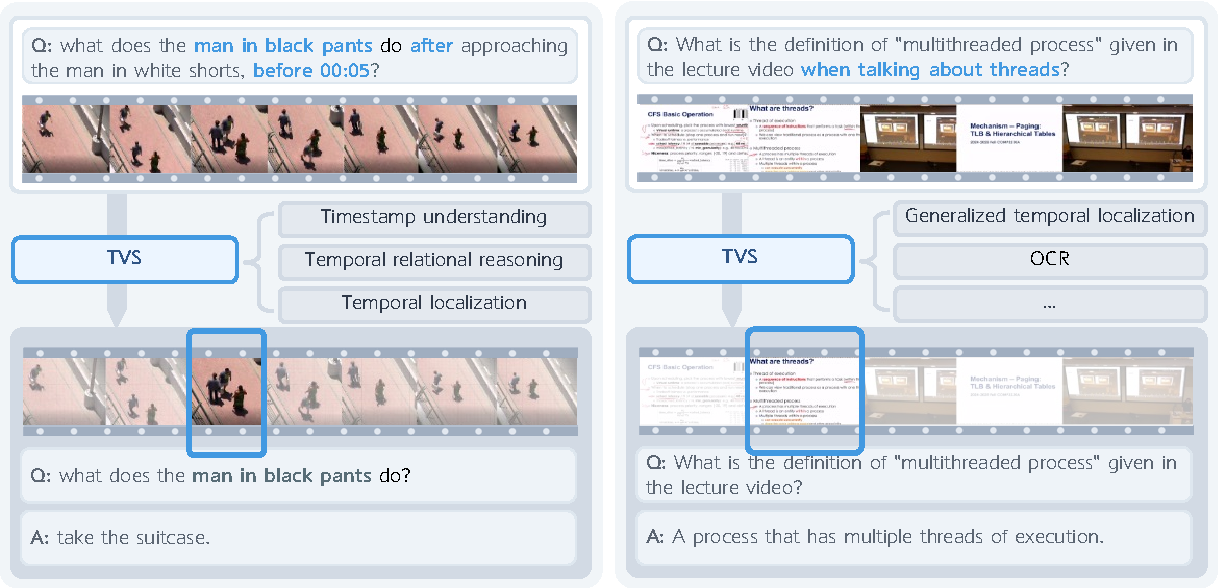
\includegraphics[width=\textwidth]{figs/tvs_task_figure12.pdf}
  \caption{Input and output example of the TVS task.\vspace{-10pt}}
  \label{fig:tvs_task_figure}
\end{figure*}

The main contributions of this work are summarized below:
\begin{itemize}
[leftmargin=*,topsep=-1pt,itemsep=0ex]
\item We propose a novel task, temporal visual screening (TVS), and introduce the ReSimplifyIt framework as a model-agnostic 
% multi-agent
plug-in 
% that can be attached to
compatible with
any existing Video-QA pipelines.
\item We propose a benchmark YouCookII-TVS for the TVS task, (which comprises XX Hours of videos and XX questions).
\item We quantitatively evaluate the impact of temporal visual screening in Video QA. \hide{\yi{Why synthesize the benchmark? Bullet point can be briefly elaborated a bit more to make intellectually exciting here} \uky{re: Have split into two points and added one-sentence elaboration above}}
\item Our method brings considerable performance boost to multiple strong baselines over various Video QA benchmarks (over 10\% absolute gain). \hide{\yi{Add concrete numerical gain}\uky{done}}

\end{itemize}

 \hide{\jiateng{The figure is not clear and not showing a good pipeline, we need to meet to further discuss the key motivation \& advantages of the framework, then I can re-draw the figure accordingly.}\uky{re: figure replaced, and pseudo-code added. please check} \uky{update: figure updated to workflow\_figure\_v1.png, please check}}

\begin{figure*}[t]
  \includegraphics[width=\textwidth]{figs/workflow_figure_v4.png}  
  \caption{ Snapshot examples of the workflow of our proposed ReSimplifyIt framework: (a) when a trial in a certain round fails, and; (b) when trial in a certain round succeeds. \vspace{-10pt}}
  \label{fig:workflow_figure}
\end{figure*}